\newpage
\section{Ablauf}\label{sec:ablauf}
Zur Untersuchung der Kommunikation zwischen der Geräten wird der Verkehr auf den
(W)LAN-Schnittstellen in verschiedenen Szenarien betrachtet:

\begin{enumerate}
    \setlength\itemsep{-0.5em}
    \item Jeweils eine Minute ohne Aktionen bei ein- und ausgeschalteter Konsole
    \item Ein- und Ausschalten über \textit{Hassbian}
    \item Ein- und Ausschalten über \textit{Harmony Hub}
\end{enumerate}

Da alle in den Szenarien betrachteten Verbindungen LAN-Verbindungen sind,
werden die entsprechenden Pakete über den zentralen Router des lokalen Netzwerks transportiert.
Aus diesem Grund wird der zu analysierende Netzverkehr dort mitgeschnitten.
Bei dem Router handelt es sich um eine \textit{FRITZ!Box 7560}.

\hyphenation{Wireshark}
Wie auch andere FRITZ!Boxen stellt diese unter der Adresse \nolinkurl{http://fritz.box/html/capture.html} eine Oberfläche bereit,
um Datenpakete an verschiedenen Schnittstellen mitzuschneiden und diese Paketmitschnitte
in einem für \textit{Wireshark} lesbaren Format herunterzuladen.

\begin{figure}[ht!]
    \centering
    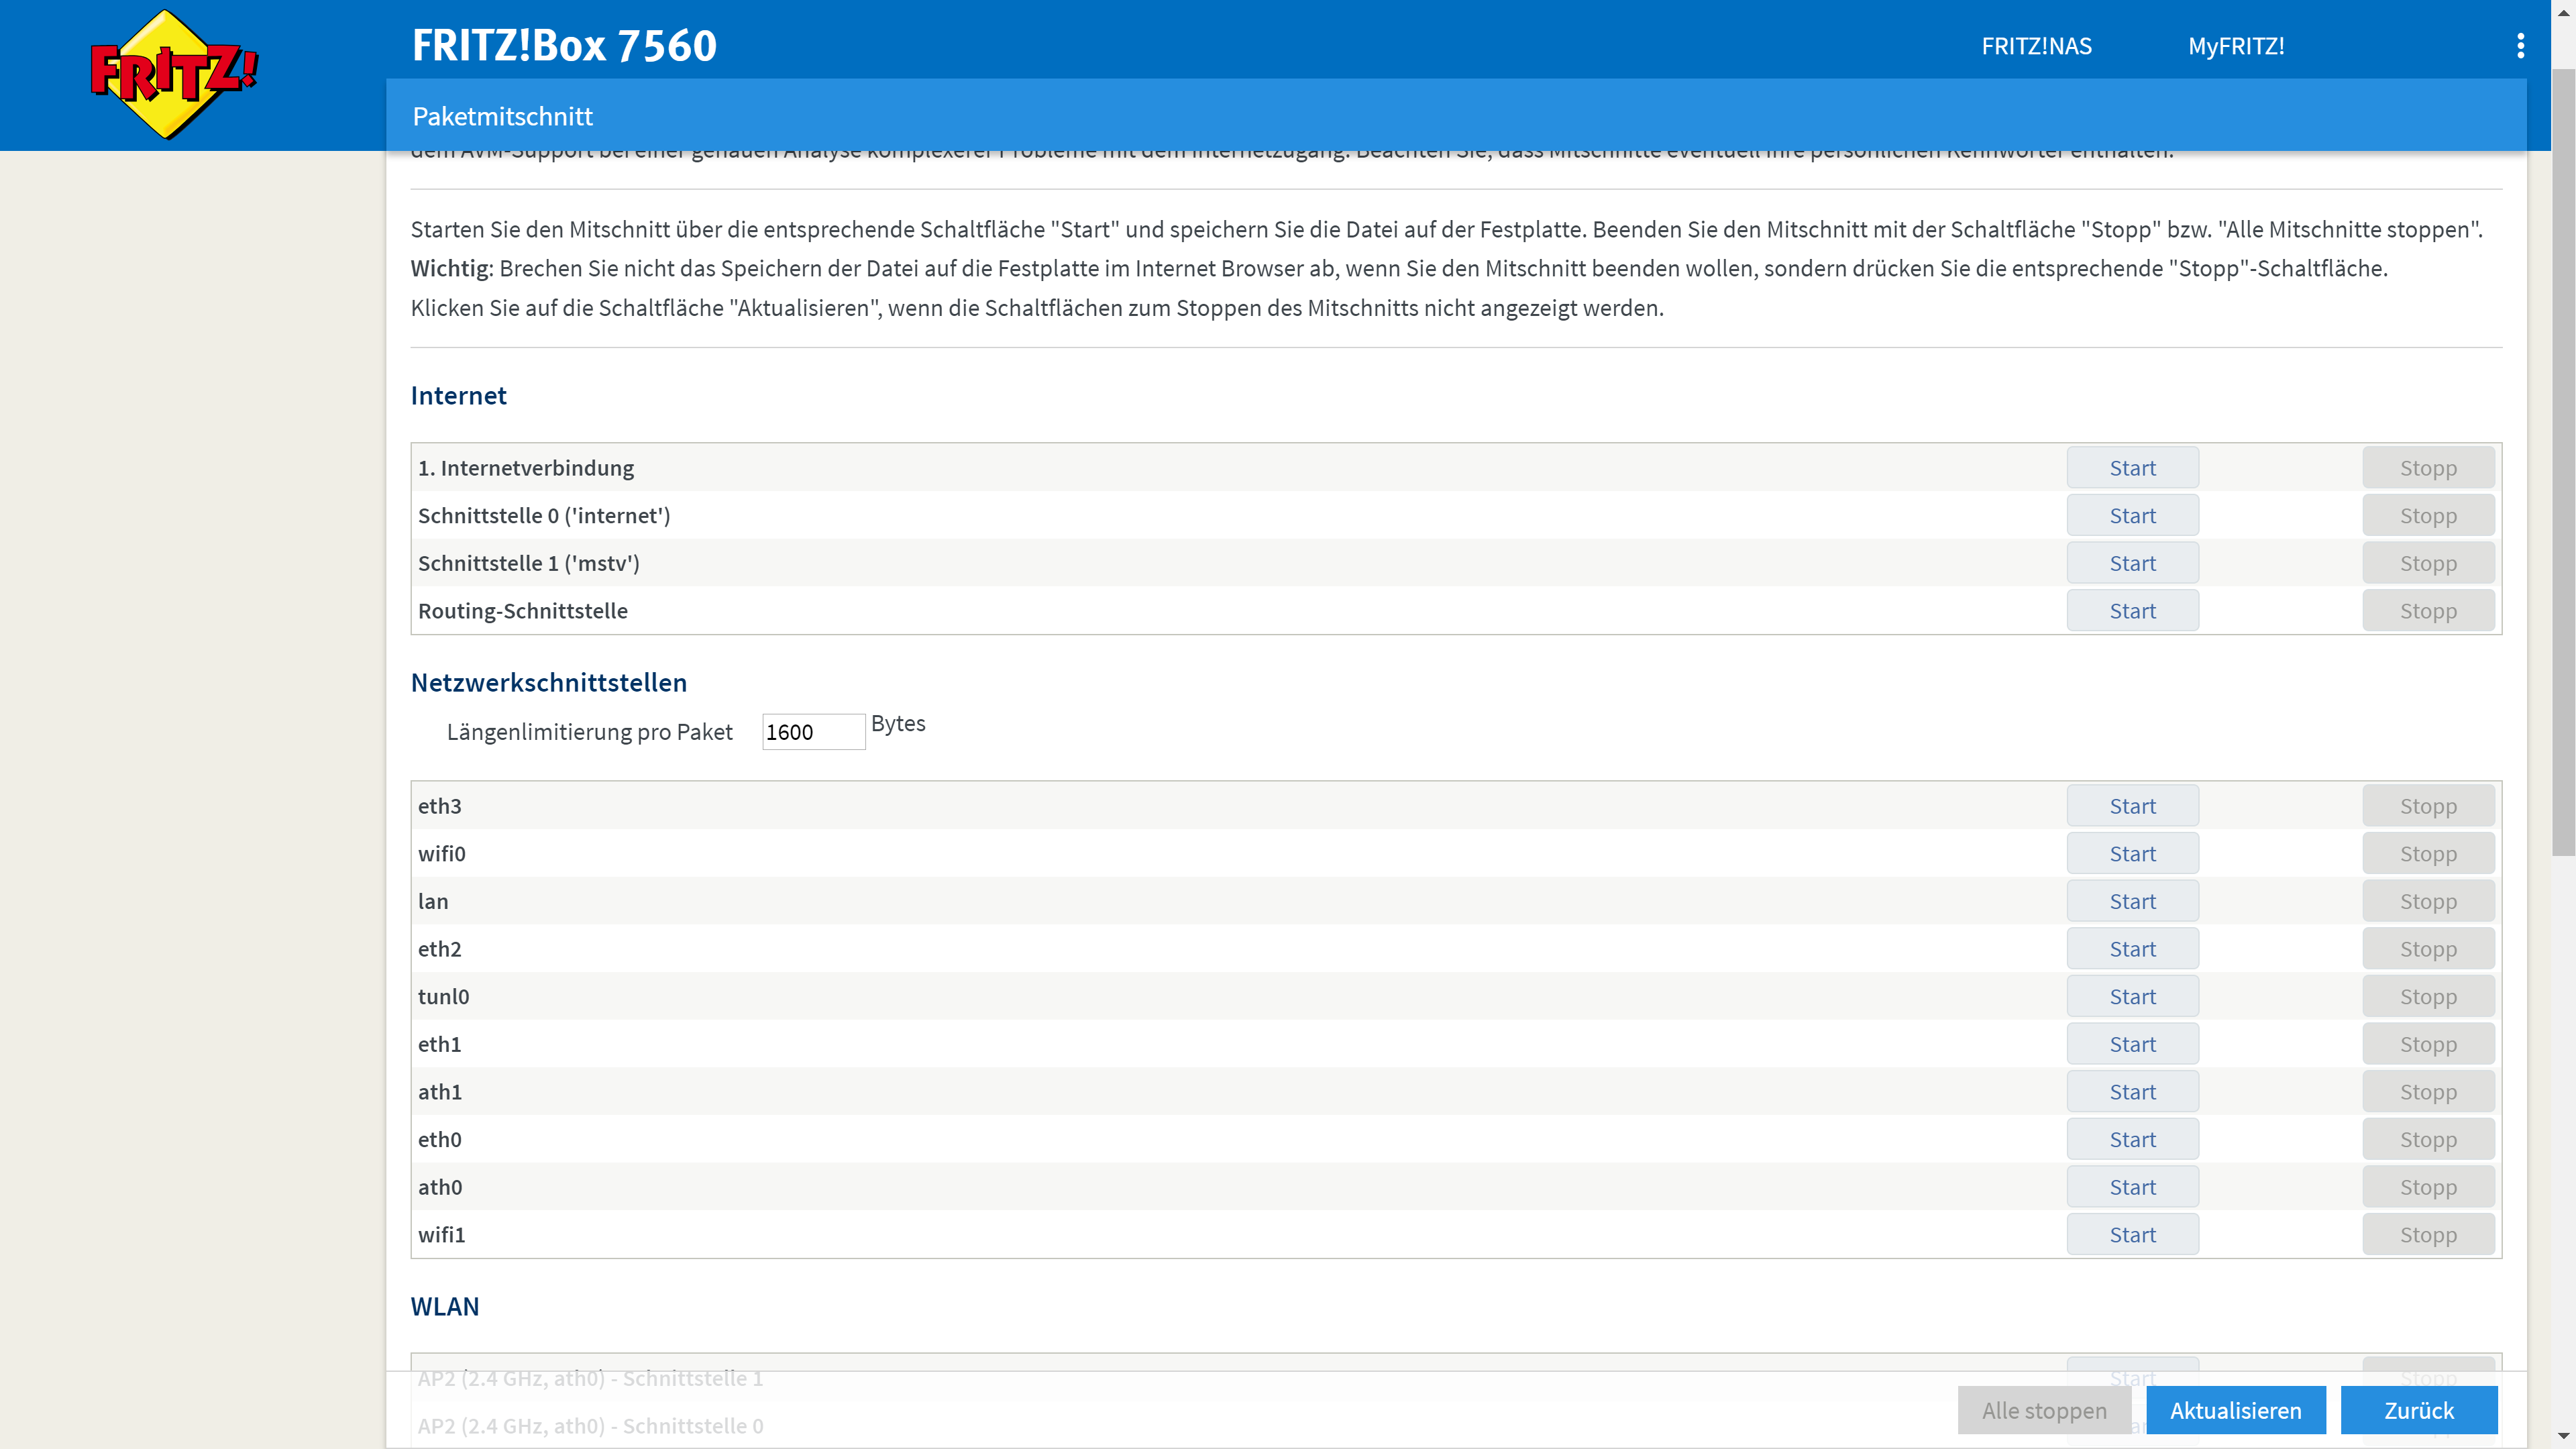
\includegraphics[width=0.75\textwidth]{fribCapture}
    \caption{FRITZ!Box Weboberfläche für Paketmitschnitte}\label{fig:fribCapture}
\end{figure}

Das Erfassen der Pakete der Szenarien geschieht nach folgendem Muster:
\begin{enumerate}
    \setlength\itemsep{-0.5em}
    \item Starten des Paketmittschnitts auf \texttt{ath0}
    \item Durchführen des Szenarios
    \item Beenden des Paketmittschnitts
    \item Öffnen des Mitschnitts mit \textit{Wireshark} und Filtern der relevanten Pakete
    \item Speichern des gefilterten Mitschnitts zur späteren Analyse
\end{enumerate}